\section{Attachements}
\subsection{Vorbereitung}
In der Versuchsvorbereitung wurden mit Matlab der IIR-Filterentwurf untersucht. Dabei wurden die zwei Filtertypen, elliptisch und Chebychev mit den Spezifikationen siehe Aufgabenbeschreibung simuliert. Für die spätere Implementierung auf einen DSP wurden die resultierenden Übertragungsfunktionen auf Systeme 2. Ordnung reduziert. Die Verstärkungsfaktor g wird dabei auf die einzelnen Systeme 2. Ordnung gleichmäßig aufgeteilt.
\subsubsection{Attachement A}

Die Filtercharakteristik Elliptisch, Chebychev sind in der Allgemeinen und in der Kaskadenstruktur in ihrem Amplitudengang in den nachfolgenden Abbildungen Dargestellt.

\begin{figure}[h]
\centering
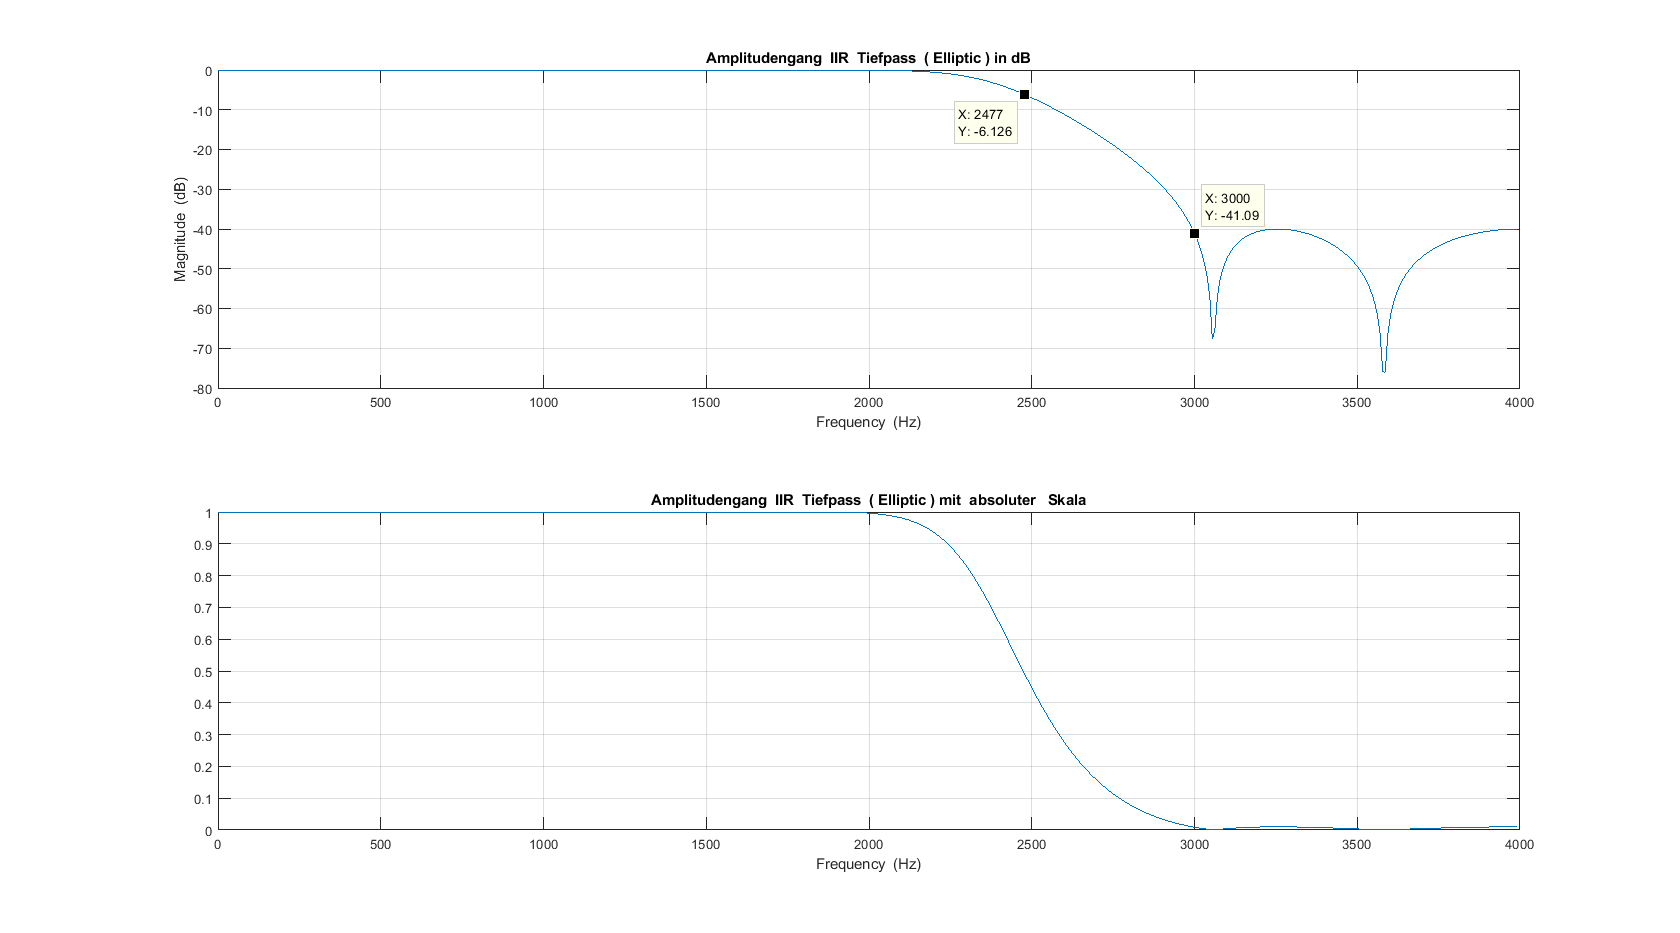
\includegraphics[width=0.7\linewidth]{Bilder/Attachment_A_ELLIP}
\caption{IIR-Filter: Elliptischer-Filtertyp - Amplitudengang}
\label{fig:Attachment_A_ELLIP}
\end{figure}
\noindent Amplitudengang des elliptischen Filtercharakteristik. Die maximale und minimale Dämpfung wird sowohl im Passband als auch im Stopband eingehalten.

\newpage

\begin{figure}[h]
	\centering
	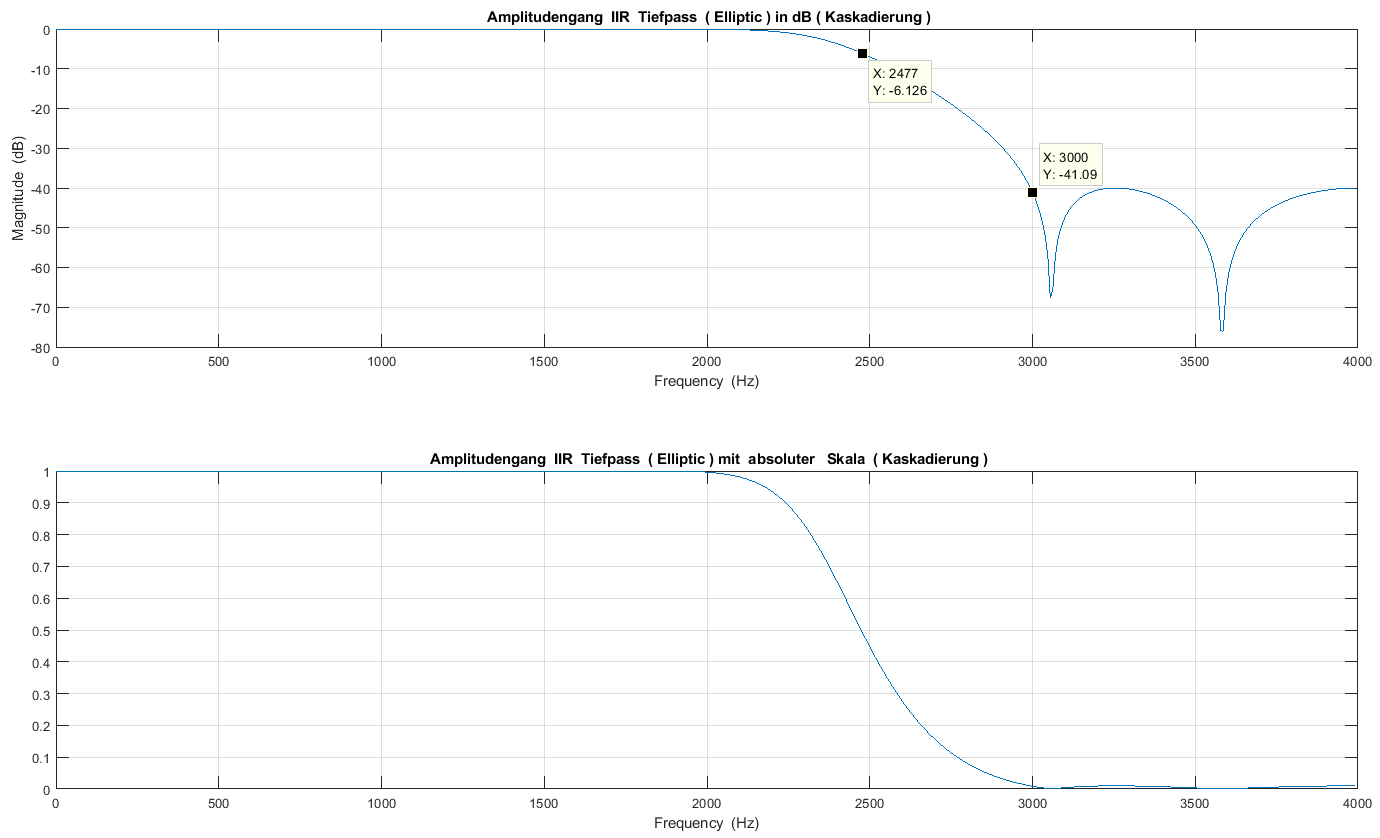
\includegraphics[width=0.7\linewidth]{Bilder/Attachment_A_ELLIP_KASKADE}
	\caption{IIR-Filter: Elliptischer-Filtertyp Kaskadenstruktur - Amplitudengang}
	\label{fig:Attachment_A_ELLIP_KASKADE}
\end{figure}
\noindent Die kaskadierte Form des elliptischen Filter zeigt den gleichen Verlauf auf wie die allgemein Form auf.



\begin{figure}[h]
\centering
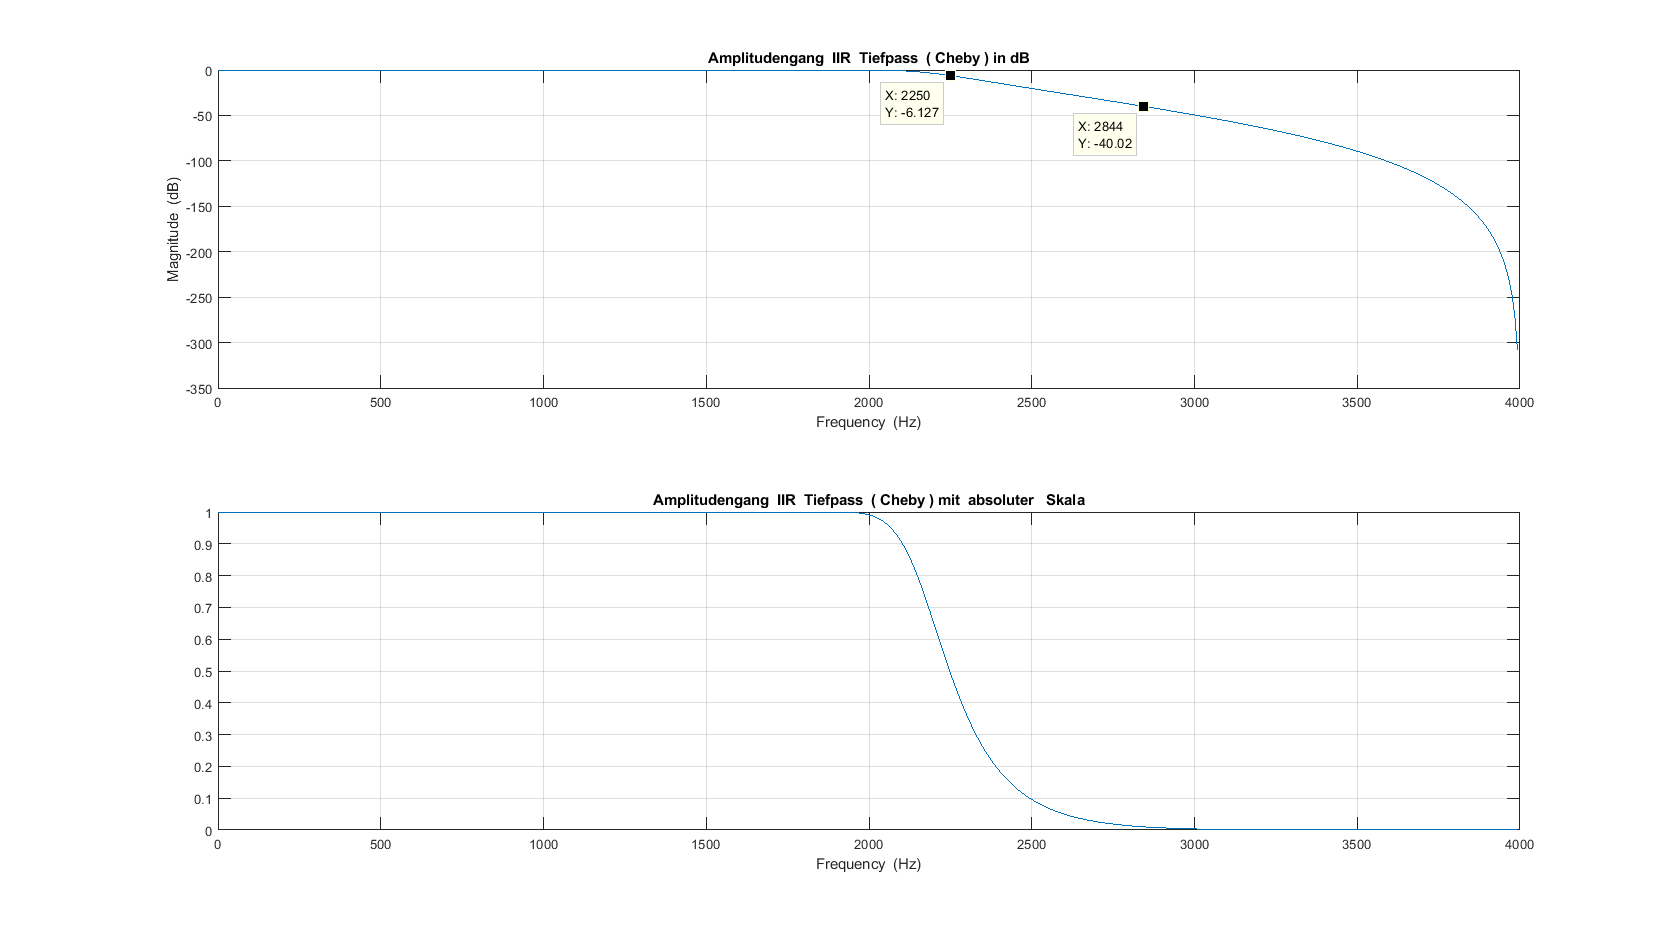
\includegraphics[width=0.7\linewidth]{Bilder/Attachment_A_CHEBY}
\caption{IIR-Filter: Chebychev-Filtertyp - Amplitudengang}
\label{fig:Attachment_A_CHEBY}
\end{figure}
\noindent Amplitudenverlauf des Chebychev Filtertyp. Die maximale Sperrdämpfung ist im Vergleich zum elliptischen Filtertyp stärker und steigt nicht mehr im Auflösungsbereich an.

\newpage

\begin{figure}[h]
\centering
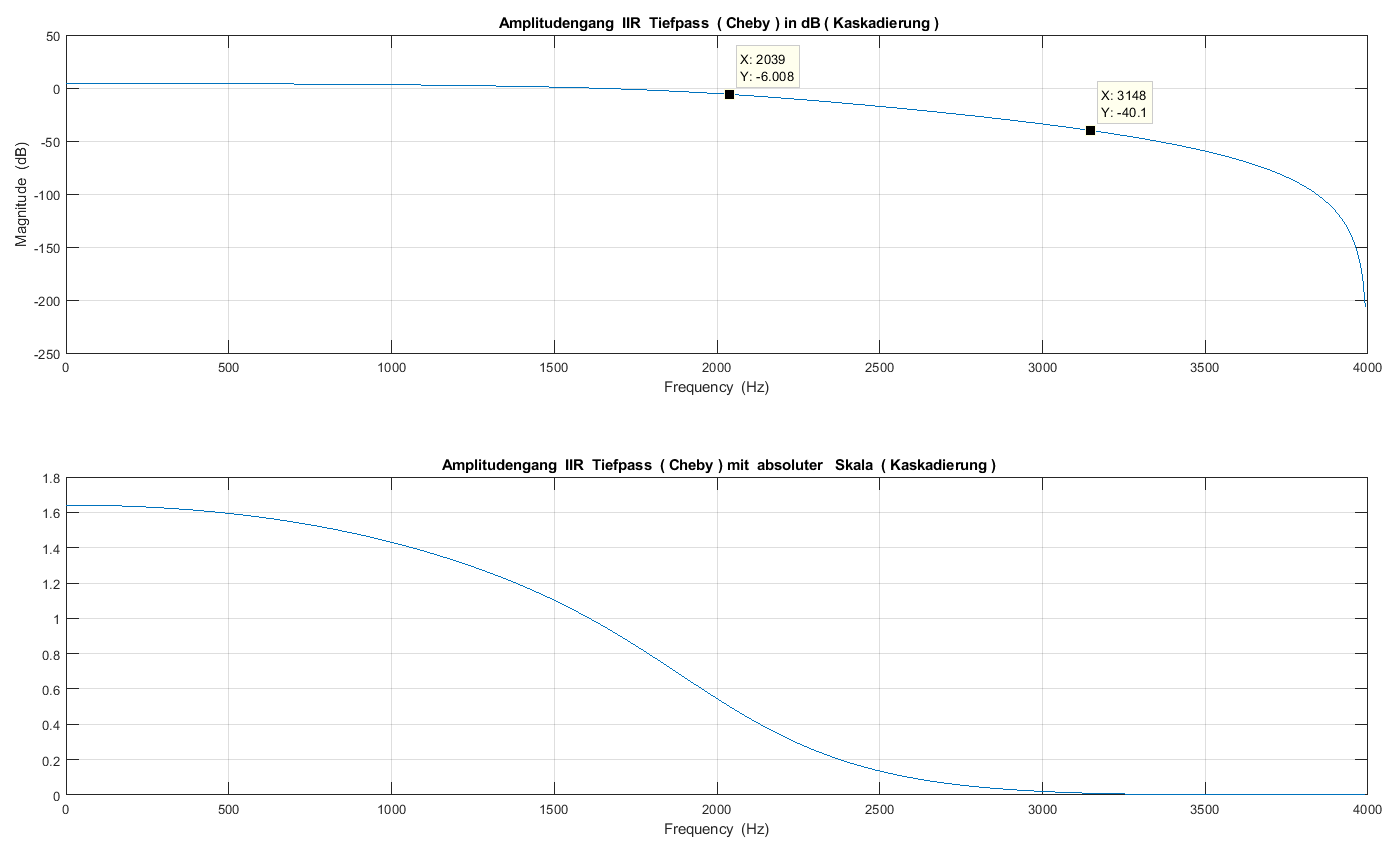
\includegraphics[width=0.7\linewidth]{Bilder/Attachment_A_CHEBY_KASKADE}
\caption{IIR-Filter: Chebychev-Filtertyp Kaskadenstruktur - Amplitudengang}
\label{fig:Attachment_A_CHEBY_KASKADE}
\end{figure}
\noindent Bei der kaskadierten Form des Chebychev-Filtertyp ist der Ripple im Passband stärker als in der allgemeinen Form und ist nicht mehr in den Spezifikationen von 0.1 db.\\

\noindent Im nachfolgenden Listing ist ein Auszug des Matlabskript zur Bestimmung des Filter Koeffizienten und Umwandlung in Systeme 2. Ordnung. Als Hinweis sei hier nochmal erwähnt, dass der Verstärkungsfaktor g bei der Überführung in Systemform 2. Ordnung auf die Koeffizienten der einzelnen Stufen gleichmäßig verteilt wird, um einen Überlauf bei der Implementierung in die Hardware zu verhindern. In der hier eingesetzten Form der Biquad wird die Verstärkung auf die b-Koeffizienten skaliert. Zusätzlich müssen noch alle Koeffizienten auf Eins normiert werden. $b_{k_{normiert}} = b_{k} \cdot 32767$\\

\begin{figure}[h]
\centering
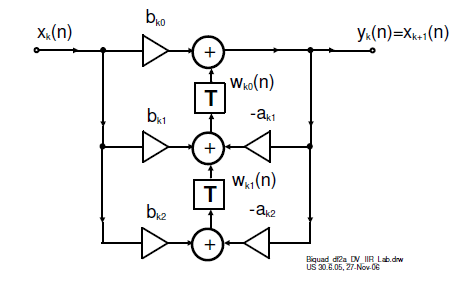
\includegraphics[width=0.7\linewidth]{Bilder/BIQUAD}
\caption{ Realisierung der k-ten Sektion 2er-Ordnung (BIQUAD)}
\label{fig:BIQUAD}
\end{figure}

\newpage

\lstinputlisting[style=c, caption={IIR-Filter Matlab Skript}, label={lst:fir_2a_koeff}]{Code/IIR_Filter_koeffizienten.m}

\noindent Koeffizienten der Filtertypen: elliptischer und Chebychev\\
Bei den Koeffizienten ist zu erkennen, dass mit einer elliptischen Implementierung zwei Biquads benötigt werden um die Spezifikationen zu erreichen. Mit der Chebychev Umsetzung werden drei Stages benötigt um diese zu erreichen.\\


\lstinputlisting[style=c, caption={IIR-Filter Koeffizienten elliptischer Typ}, label={lst:fir_2a_koeff}]{Code/IIR_ellip_LP.h}

\lstinputlisting[style=c, caption={IIR-Filter Koeffizienten elliptischer Typ}, label={lst:fir_2a_koeff}]{Code/IIR_cheby1_LP.h}



\newpage
\subsubsection{Attachement B}

\begin{figure}
\centering
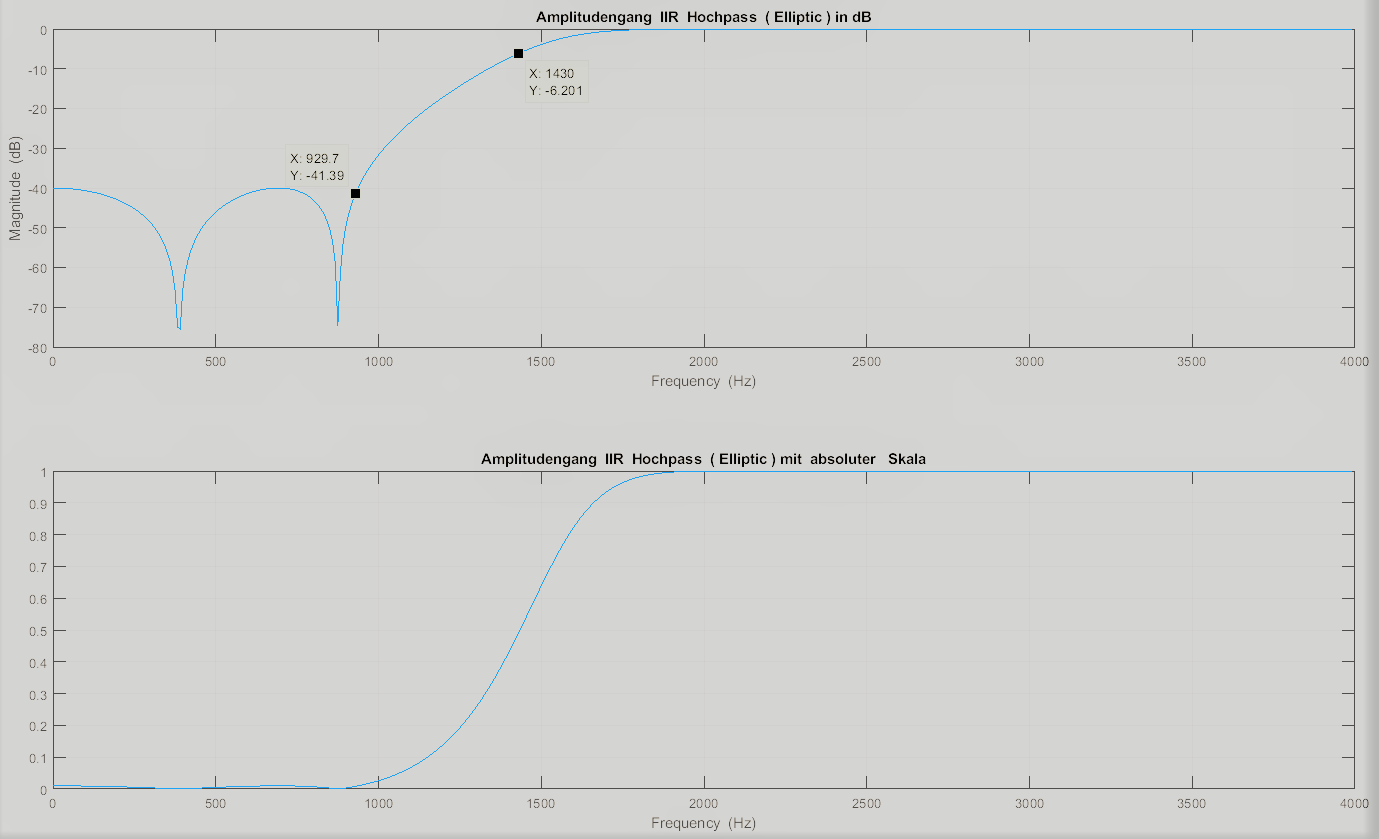
\includegraphics[width=0.7\linewidth]{Bilder/Attachment_B_ELLIP}
\caption{}
\label{fig:Attachment_B_ELLIP}
\end{figure}

\begin{figure}
\centering
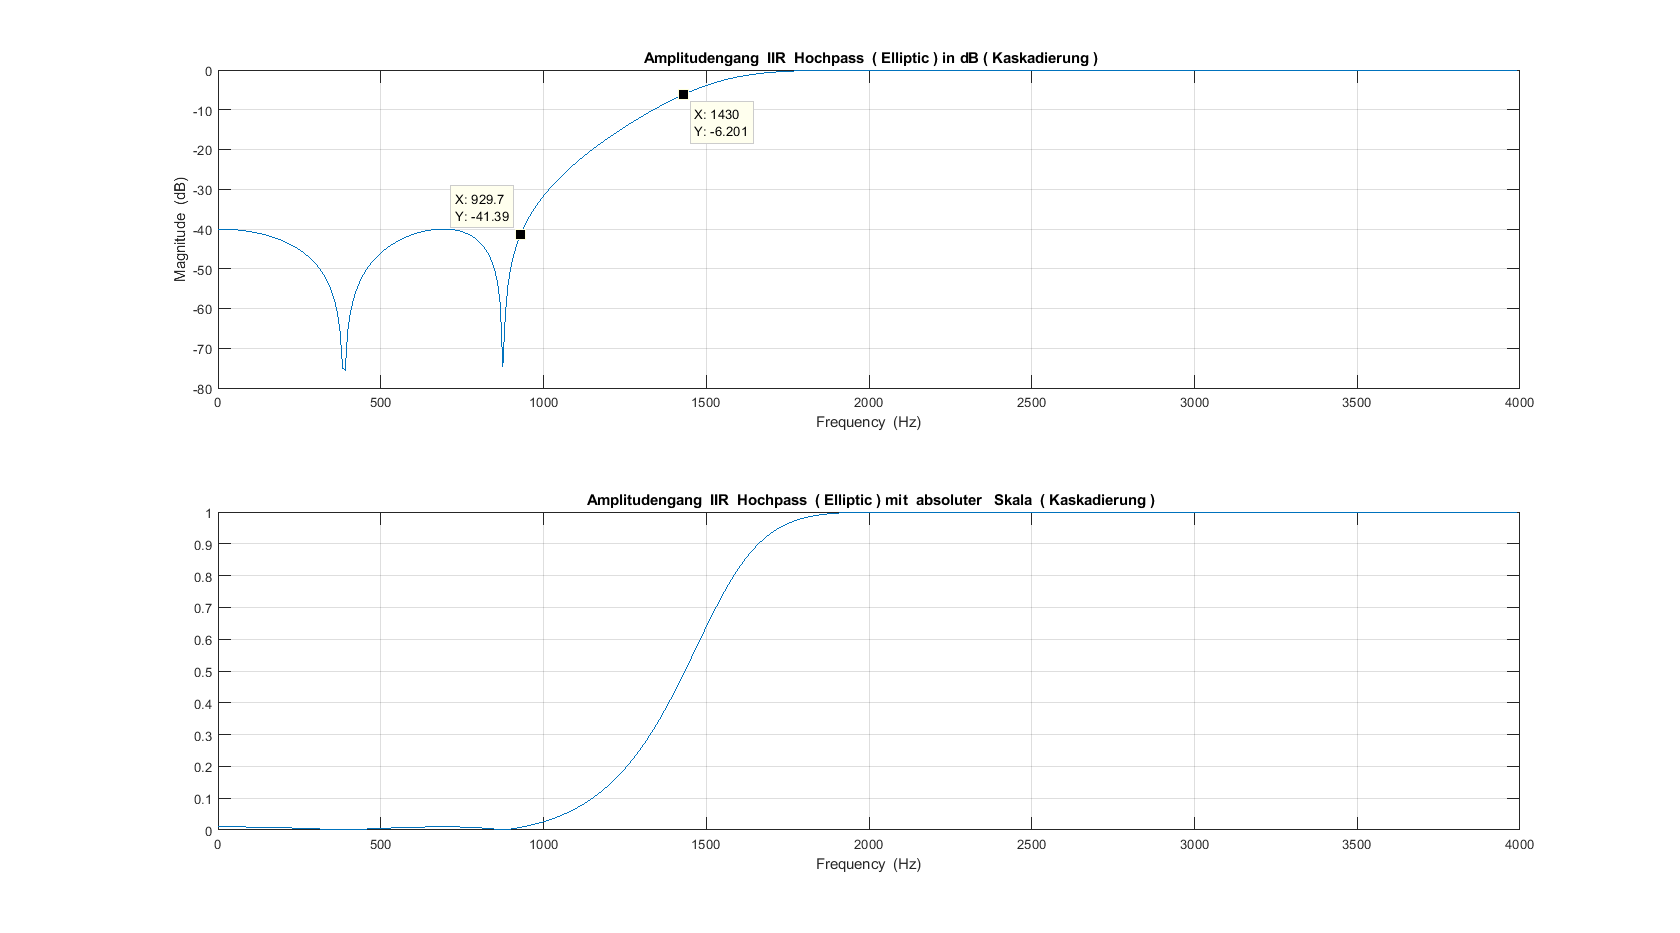
\includegraphics[width=0.7\linewidth]{Bilder/Attachment_B_ELLIP_KASKADE}
\caption{}
\label{fig:Attachment_B_ELLIP_KASKADE}
\end{figure}





\subsubsection{Attachement D}

\begin{figure}
\centering
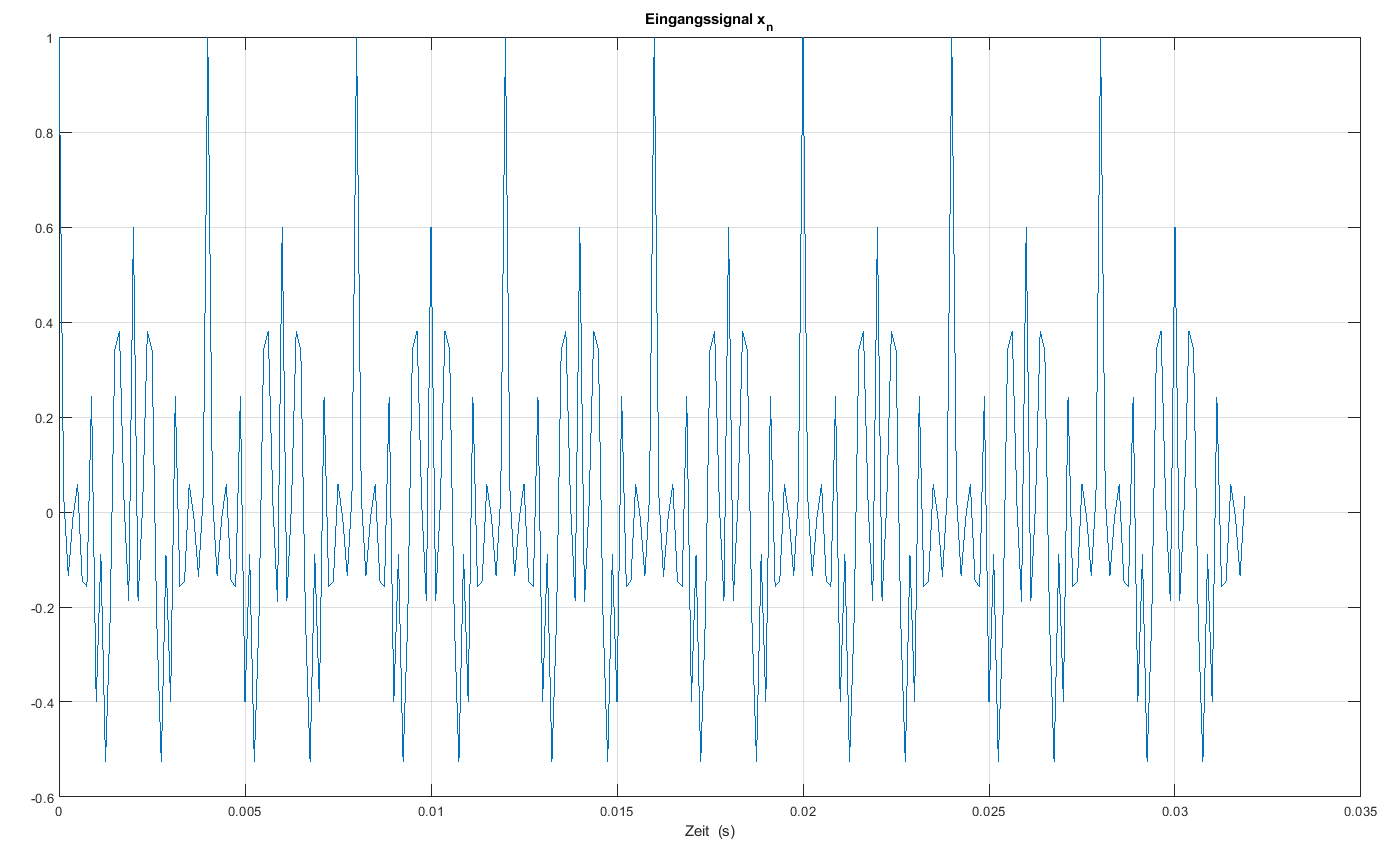
\includegraphics[width=0.7\linewidth]{Bilder/Attachment_D_Eingangszeitsignal}
\caption{}
\label{fig:Attachment_D_Eingangszeitsignal}
\end{figure}

\begin{figure}
\centering
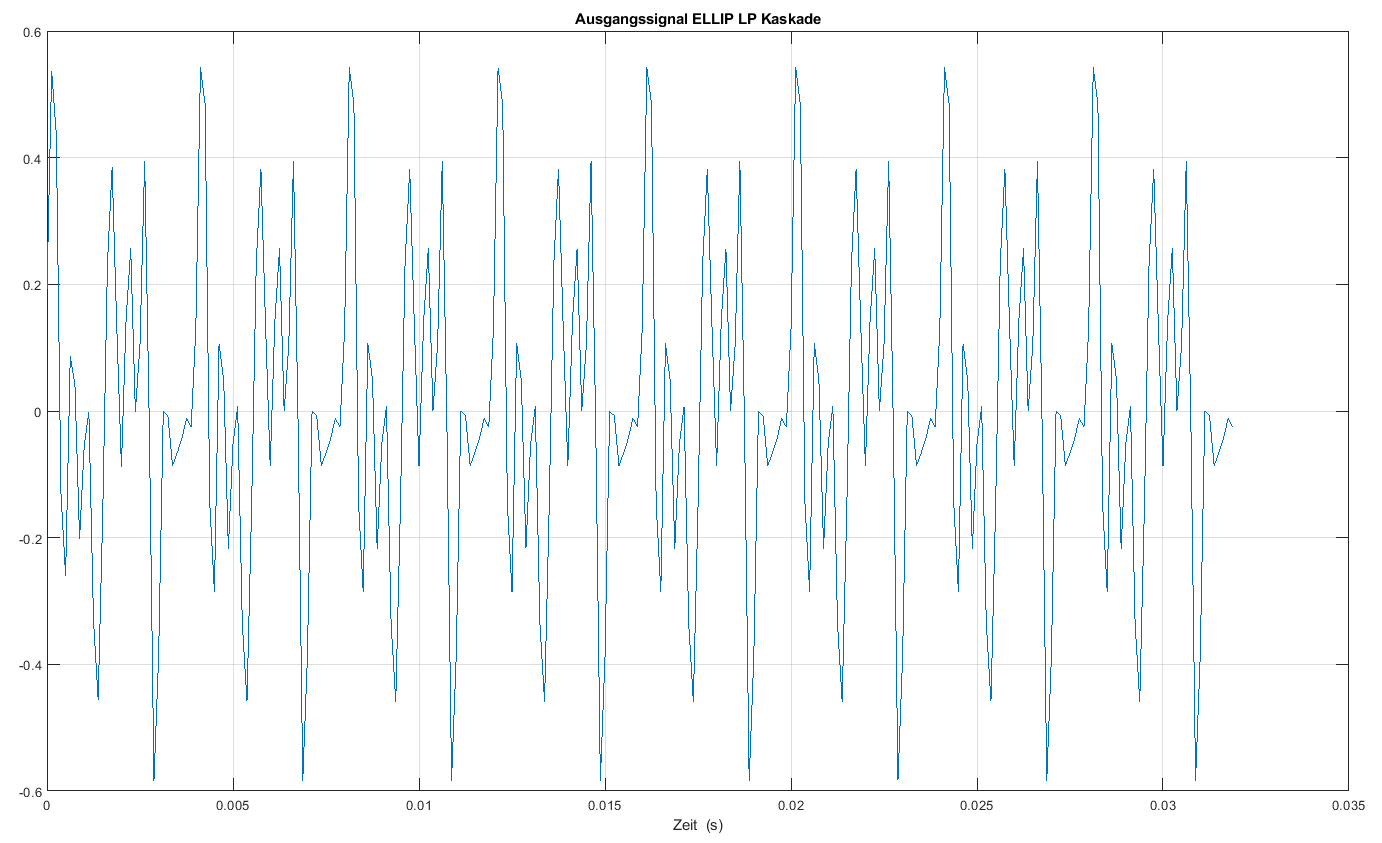
\includegraphics[width=0.7\linewidth]{Bilder/Attachment_D_Ausgangssignal_ellip_lp}
\caption{}
\label{fig:Attachment_D_Ausgangssignal_ellip_lp}
\end{figure}

\begin{figure}
\centering
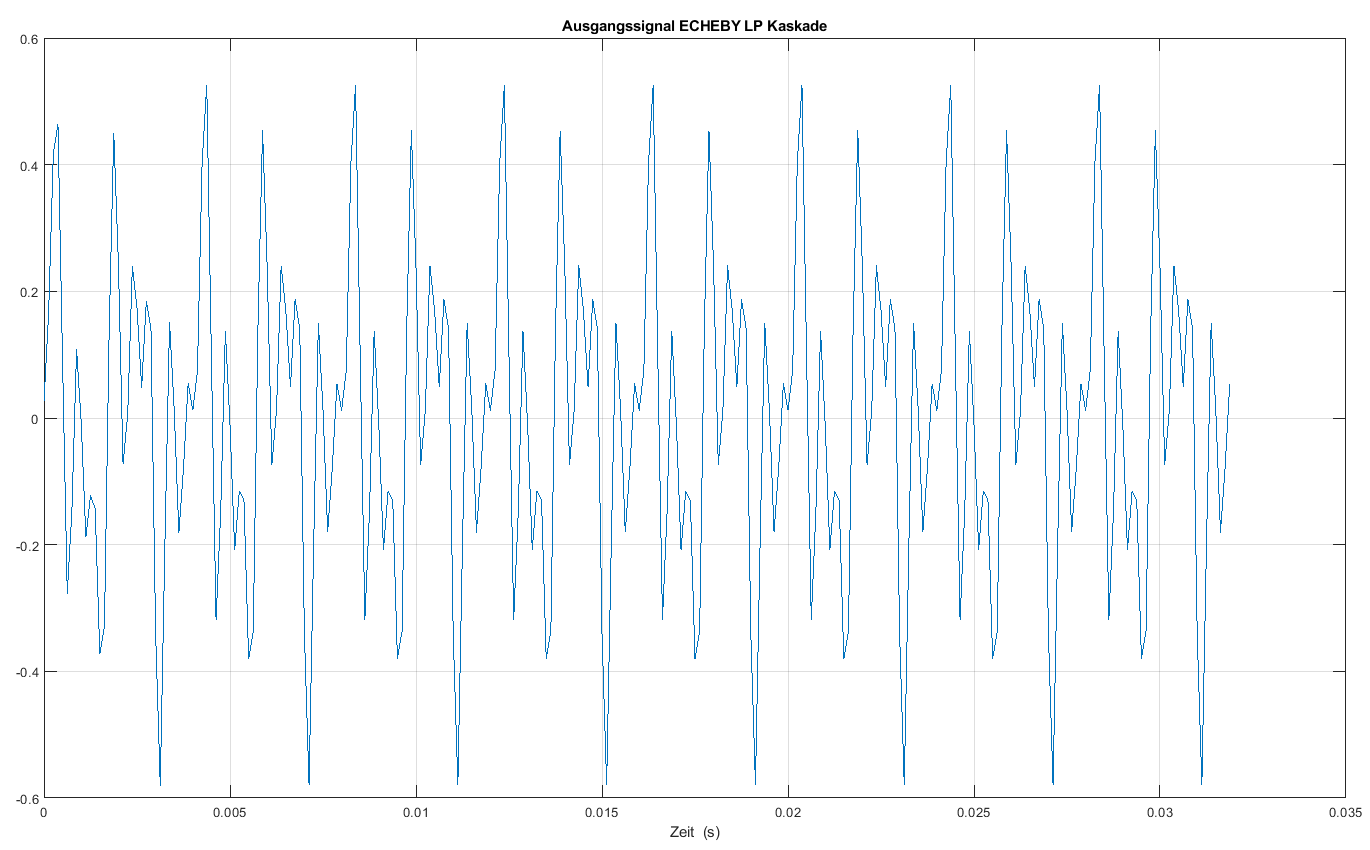
\includegraphics[width=0.7\linewidth]{Bilder/Attachment_D_Ausgangssignal_cheby_lp}
\caption{}
\label{fig:Attachment_D_Ausgangssignal_cheby_lp}
\end{figure}

\begin{figure}
\centering
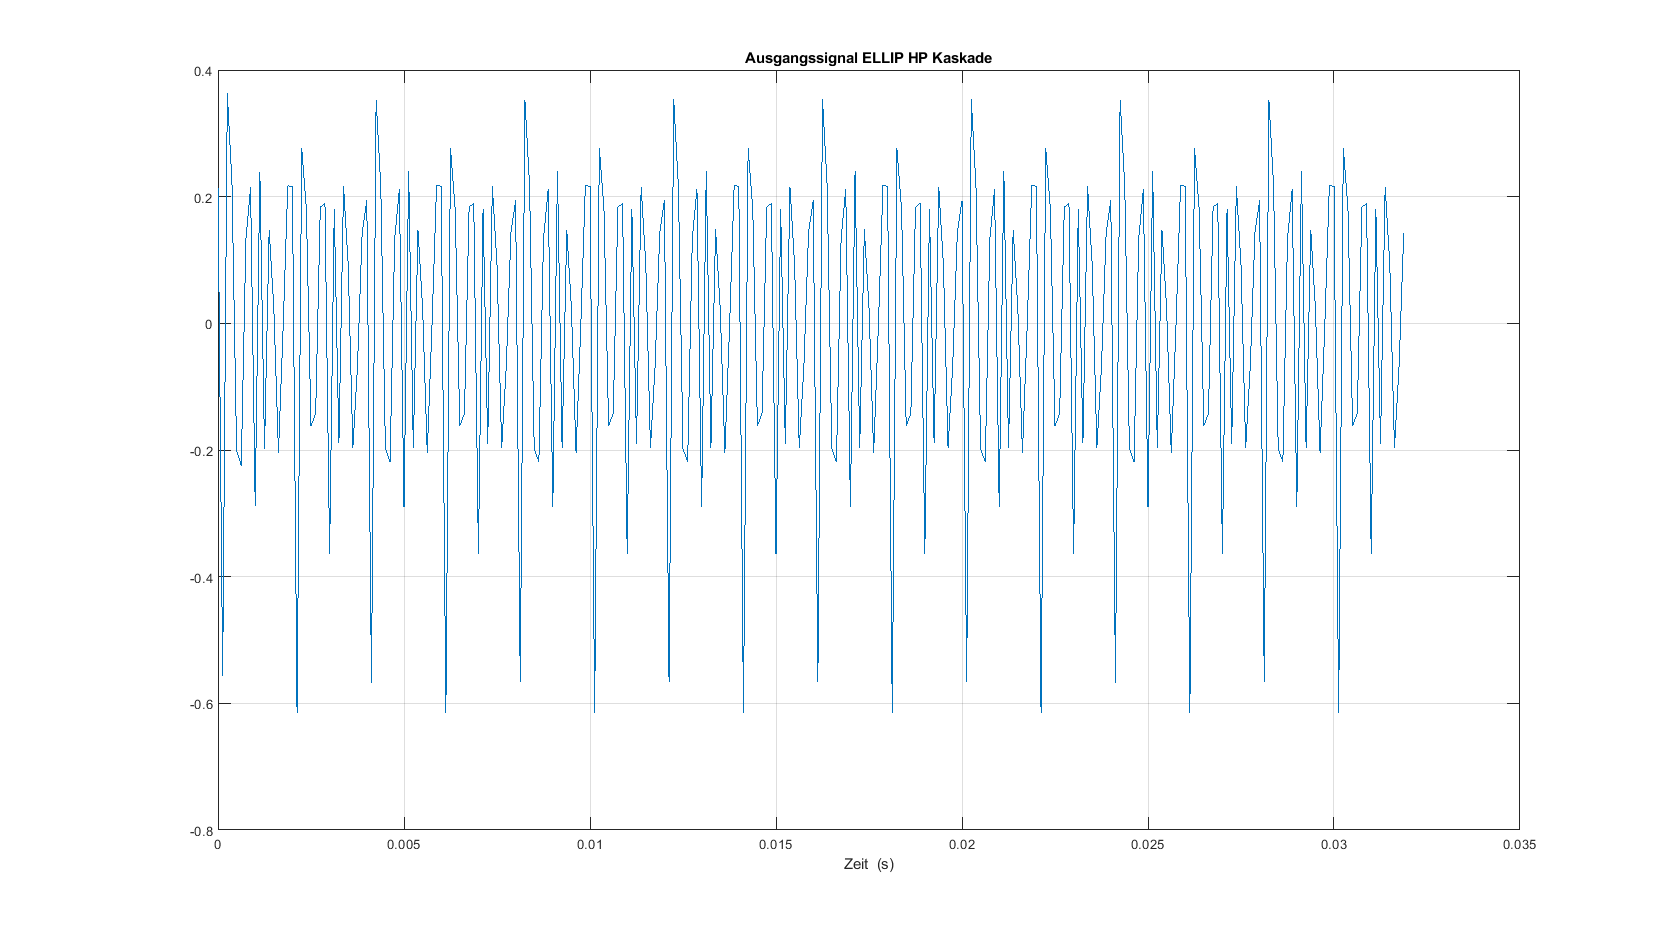
\includegraphics[width=0.7\linewidth]{Bilder/Attachment_D_Ausgangssignal_ellip_hp}
\caption{}
\label{fig:Attachment_D_Ausgangssignal_ellip_hp}
\end{figure}




\subsubsection{Attachement E}


\begin{figure}
\centering
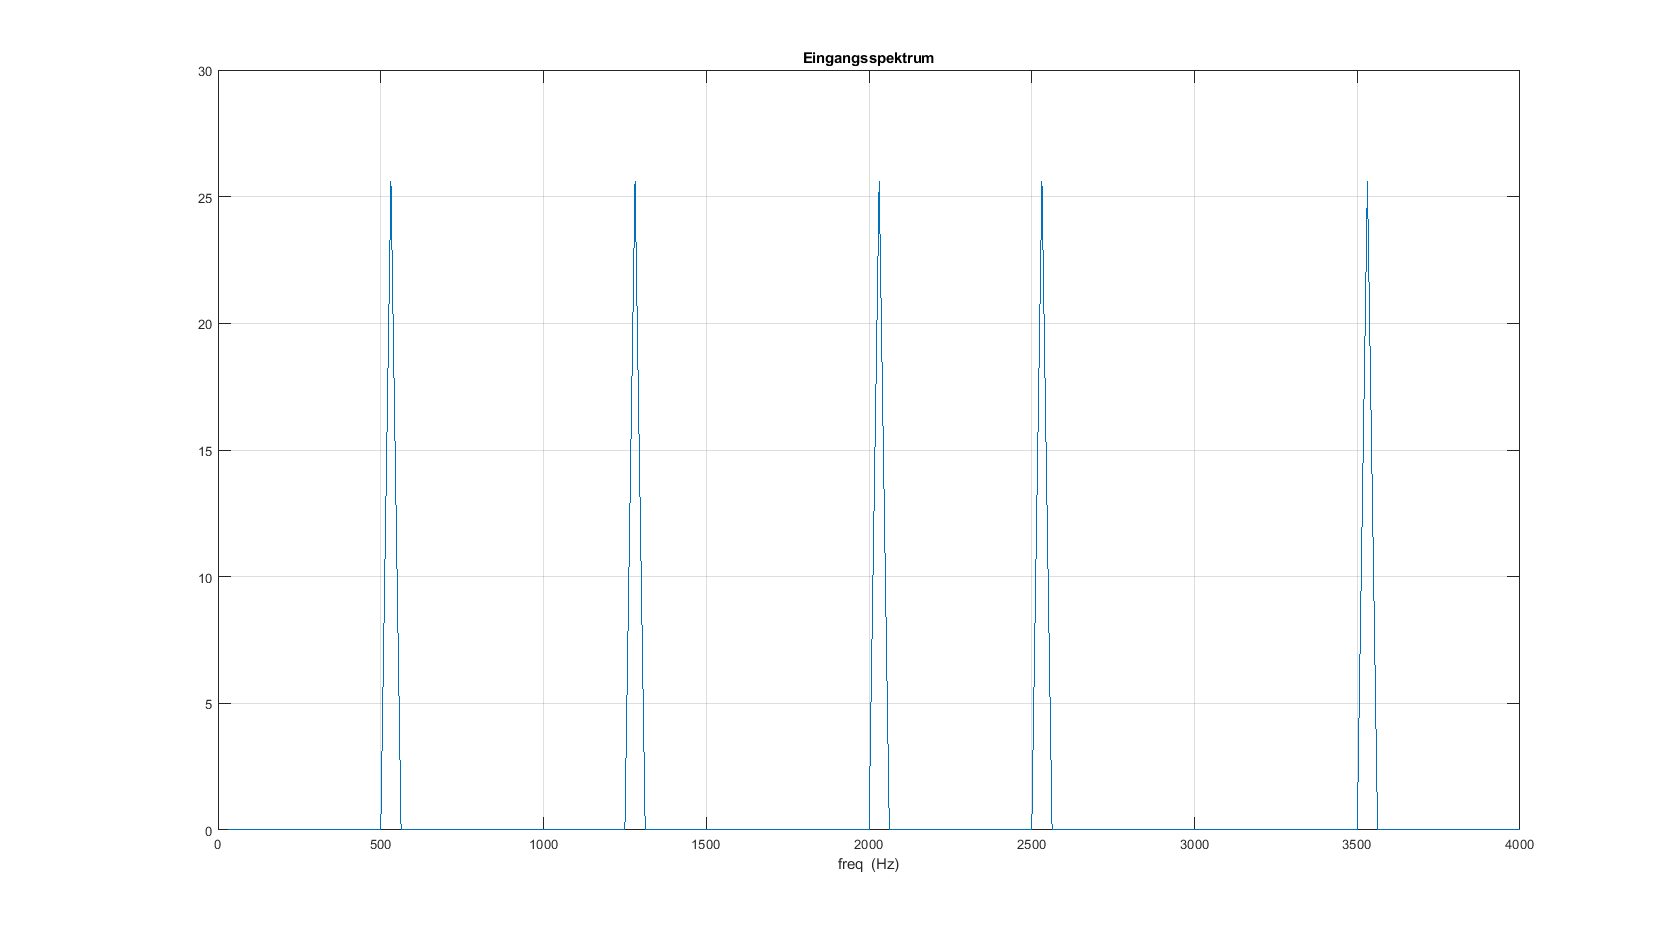
\includegraphics[width=0.7\linewidth]{Bilder/Attachment_E_Eingangsspektrum}
\caption{}
\label{fig:Attachment_E_Eingangsspektrum}
\end{figure}


\begin{figure}
\centering
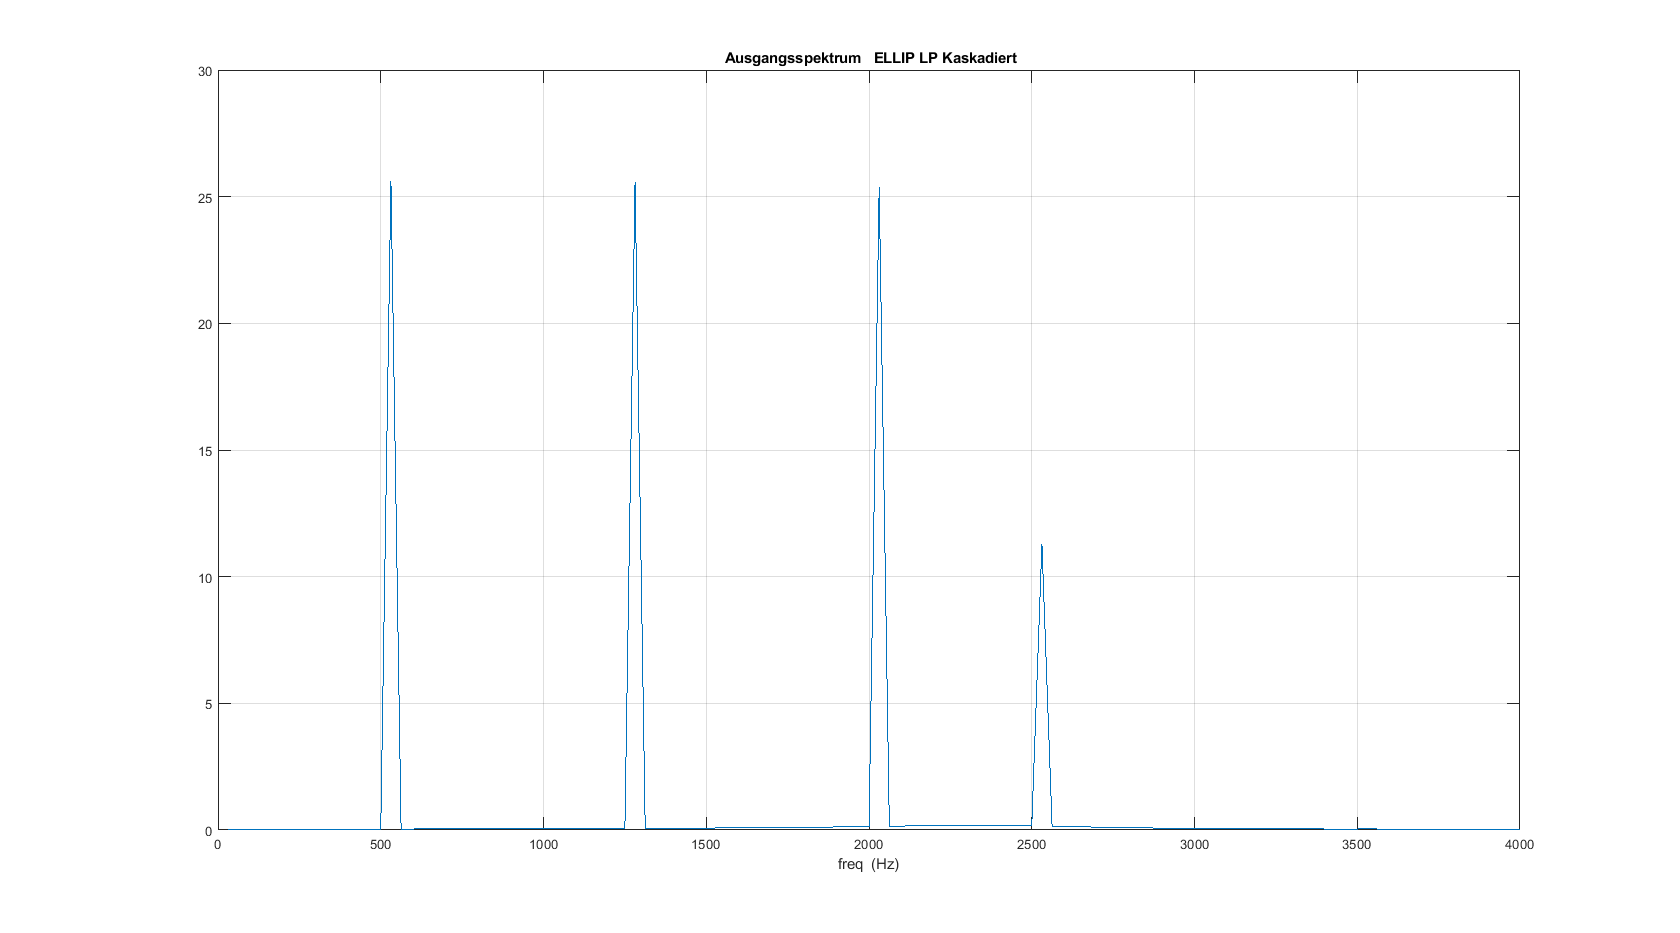
\includegraphics[width=0.7\linewidth]{Bilder/Attachment_E_ELLIP_LP_Spektrum}
\caption{}
\label{fig:Attachment_E_ELLIP_LP_Spektrum}
\end{figure}


\begin{figure}
\centering
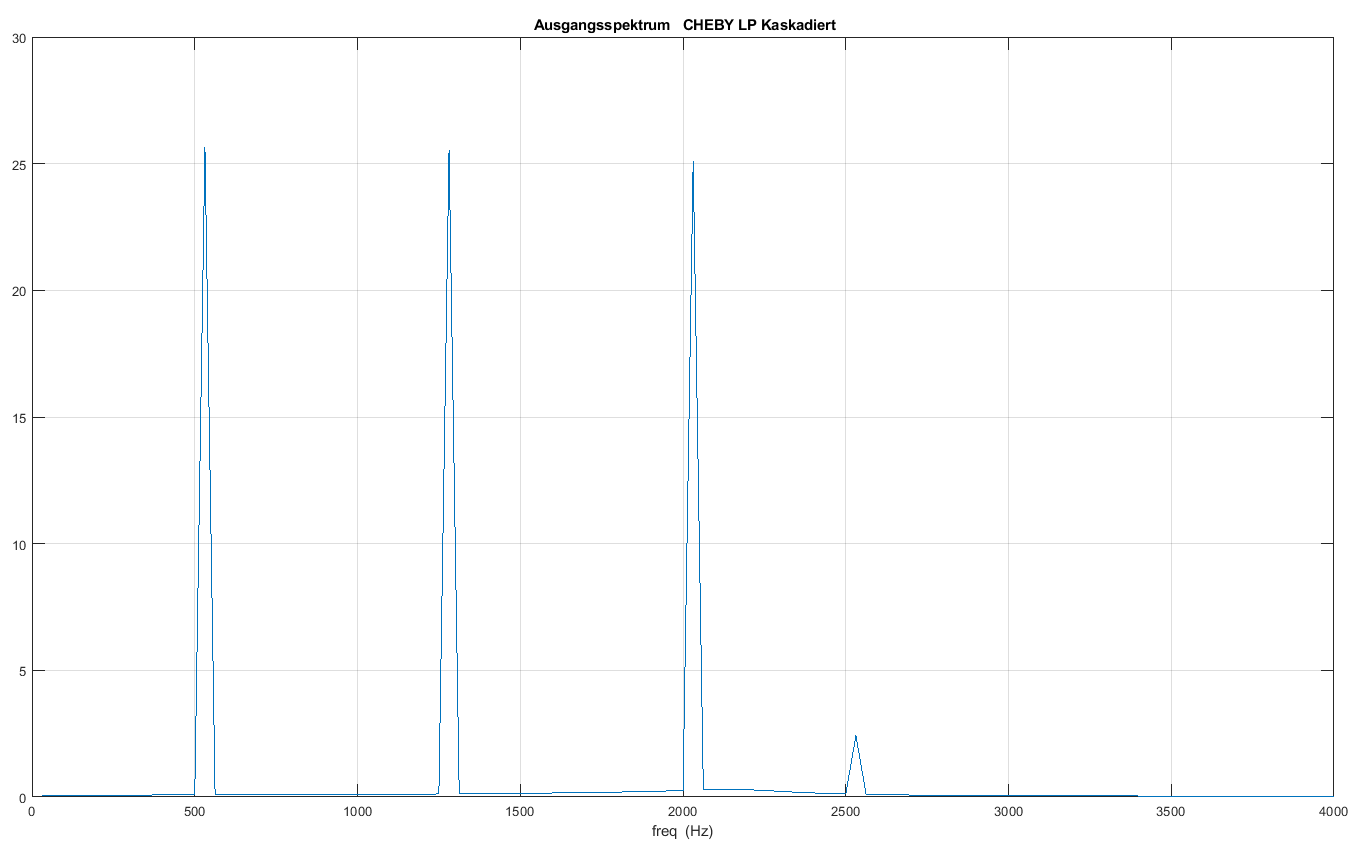
\includegraphics[width=0.7\linewidth]{Bilder/Attachment_E_CHEBY_LP_Spektrum}
\caption{}
\label{fig:Attachment_E_CHEBY_LP_Spektrum}
\end{figure}

\begin{figure}
\centering
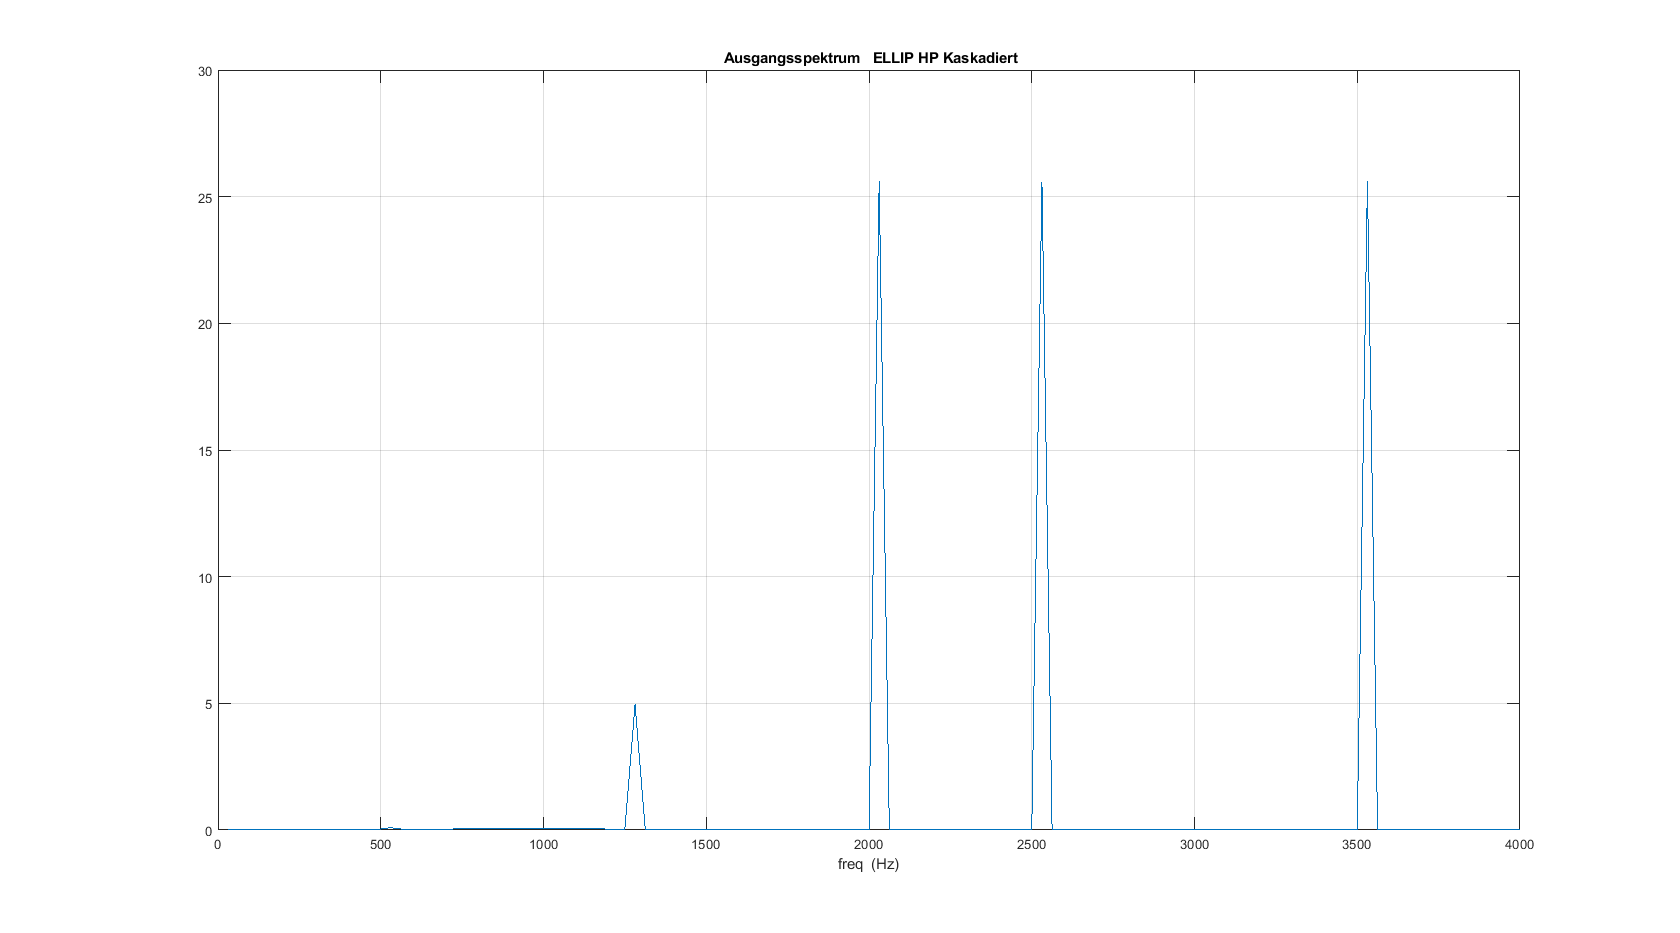
\includegraphics[width=0.7\linewidth]{Bilder/Attachment_E_ELLIP_HP_Spektrum}
\caption{}
\label{fig:Attachment_E_ELLIP_HP_Spektrum}
\end{figure}



\subsection{Lowpass filter}
\subsubsection{Attachement F}

	\begin{figure}[h]
		\centering
		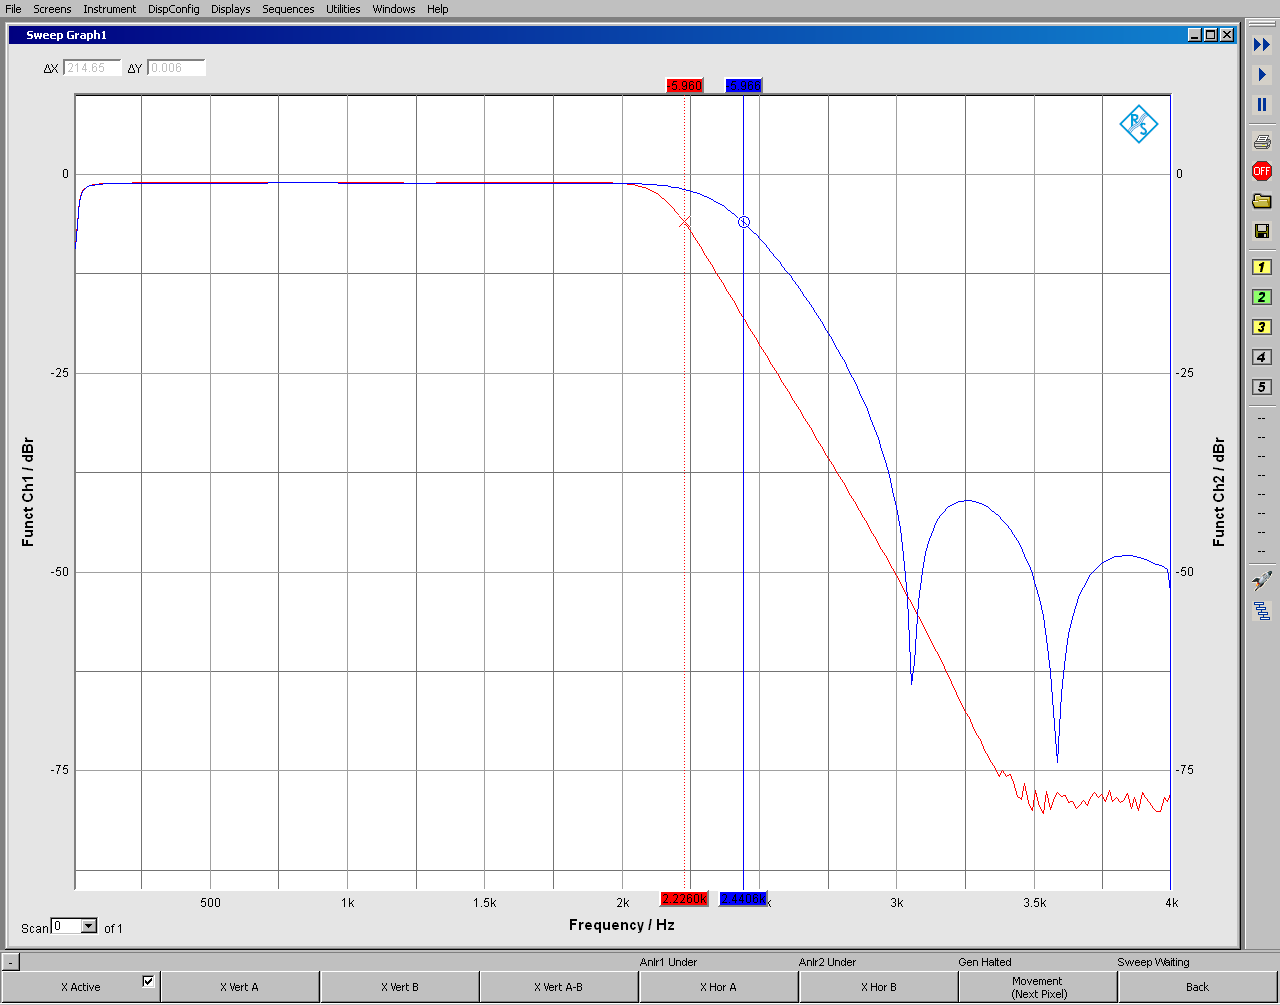
\includegraphics[width=0.8\linewidth]{Bilder/EllipCheby}
		\caption{Blau: Elliptisches IIR TP-Filter | Rot: Chebychev IIR TP-Filter}
		\label{fig:EllipCheby}
	\end{figure}
	
\noindent Der linke Ausgang lieferte das mit einem elliptischen TP-Filter gefilterte Eingangssignal (blau), der rechte Ausgang lieferte das mit einem Chebychev-TP-Filter gefilterte Eingangssignal (rot). Ein Frequenzsweep von 0 .. 4kHz wurde für die Messungen durchgeführt. Die Filterrealisierung geschah jeweils über k kaskadierter Biquads zweiter Ordnung. Für das elliptische Filter war k = 2, für Chebychev war k = 3.

\subsubsection{Attachement G}


\subsection{Hochpass - Tiefpass - Weichenfilter}


\subsection{Modifiziertes elliptisches Tiefpassfilter}
\subsubsection{Attachement H}


\subsubsection{Attachement J}


\subsubsection{Attachement K}

	\begin{figure}[h]
		\centering
		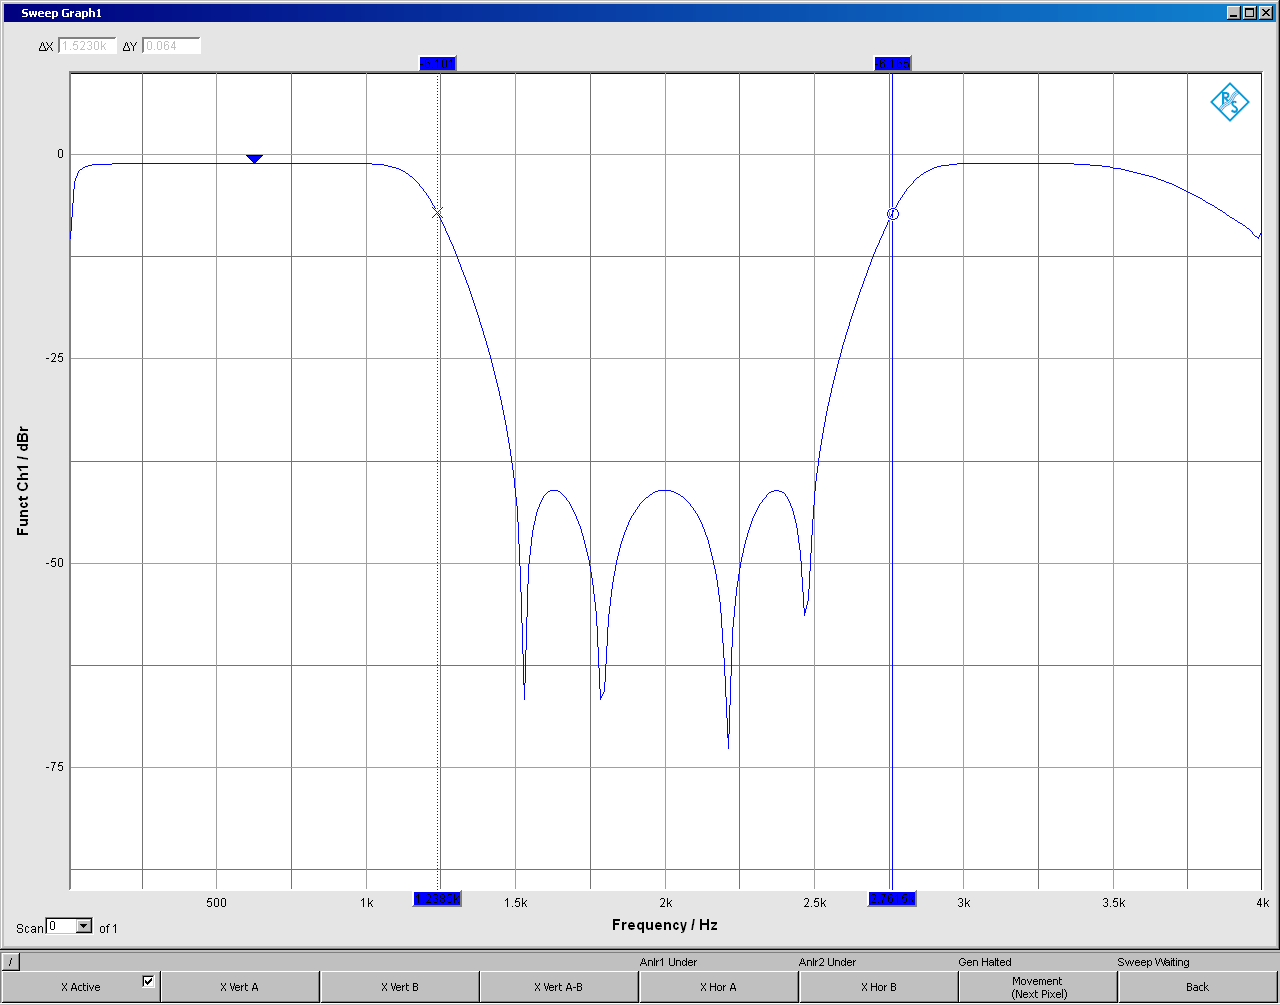
\includegraphics[width=0.7\linewidth]{Bilder/ellip2T}
		\caption{Frequenzgang modifiziertes Tiefpassfilter $|T| \rightarrow |2T|$}
		\label{fig:ellip2T}
	\end{figure}
